\title{Milestone 1}
\author{Singularity Software}
\date{\today}

\documentclass[12pt]{article}
\usepackage[a4paper]{geometry}
\usepackage{makeidx}
\usepackage{lscape}
\usepackage{amsmath}
\usepackage{graphicx}
\usepackage[final]{pdfpages}

\geometry{top=1.0in, bottom=1.0in, left=1.0in, right=1.0in} % Sets the margins

\setlength{\parindent}{0pt} % Fixes the paragraph spacing problem

\renewcommand*\arraystretch{1.5}

\begin{document}

\begin{center}
	\LARGE{Milestone 2} \\
	\Large{\textit{Singularity Software}} \\
	\vspace{.05in}
	\normalsize{\today} \\
\end{center}

\section*{Sprint 1 Backlog}
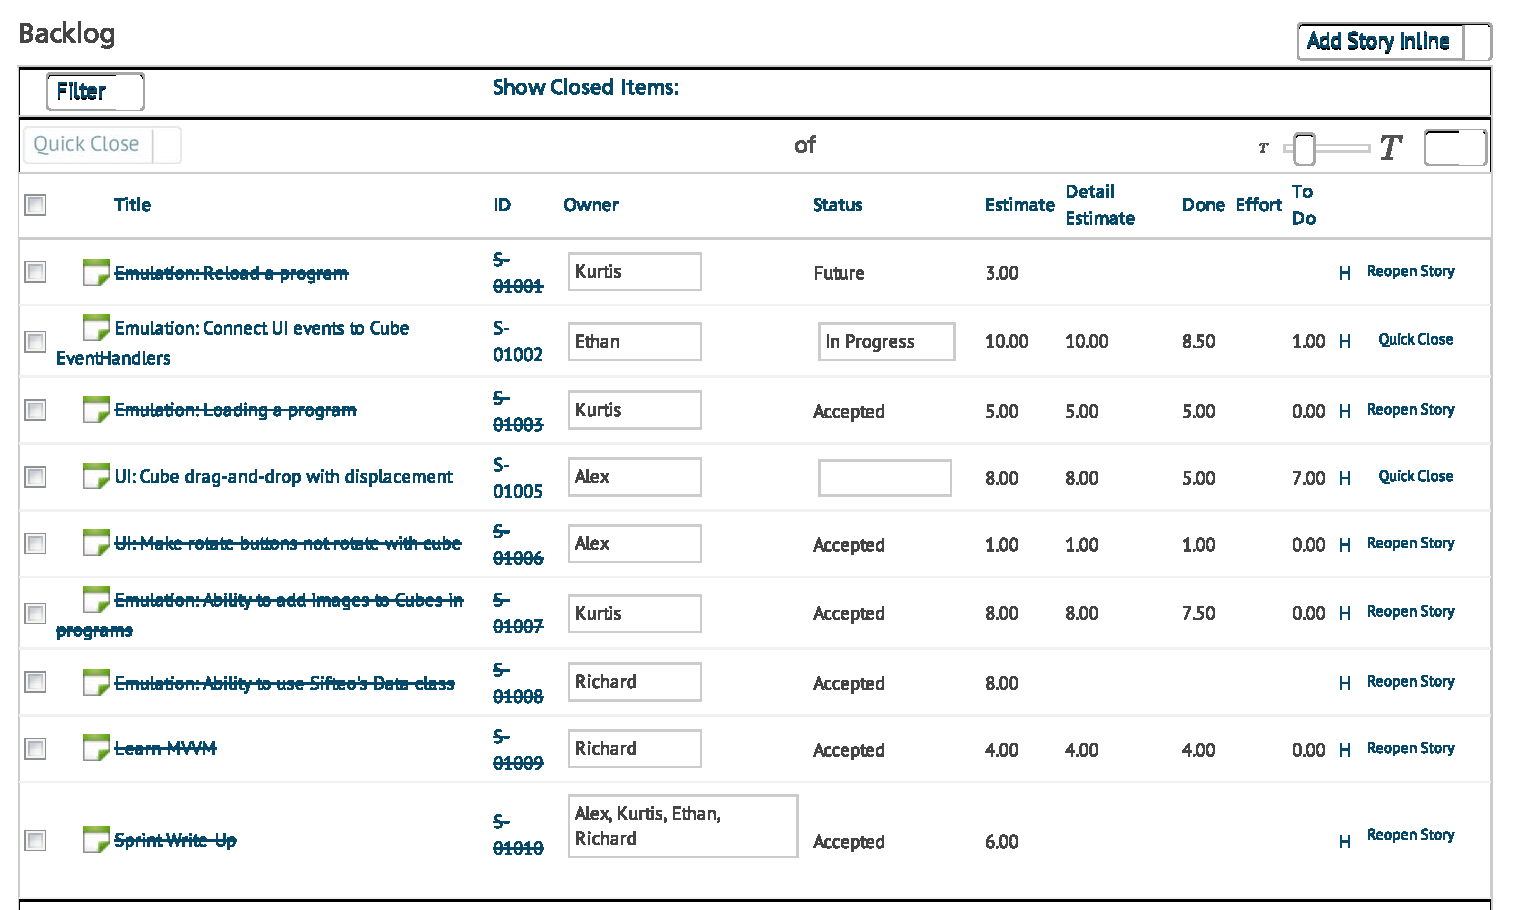
\includegraphics[scale=.63]{pdfs/MS2VersionOne/OldSprintBacklog_cropped.pdf}

The CubeEventHandlers are being tested for accuracy in the next sprint, and that task will be approved when they are completely tested. The drag-and-drop with replacement feature is in progress but unlikely to be finished for this sprint, so it will carry over to the next sprint.

\clearpage

\section*{Sprint 2 Backlog}
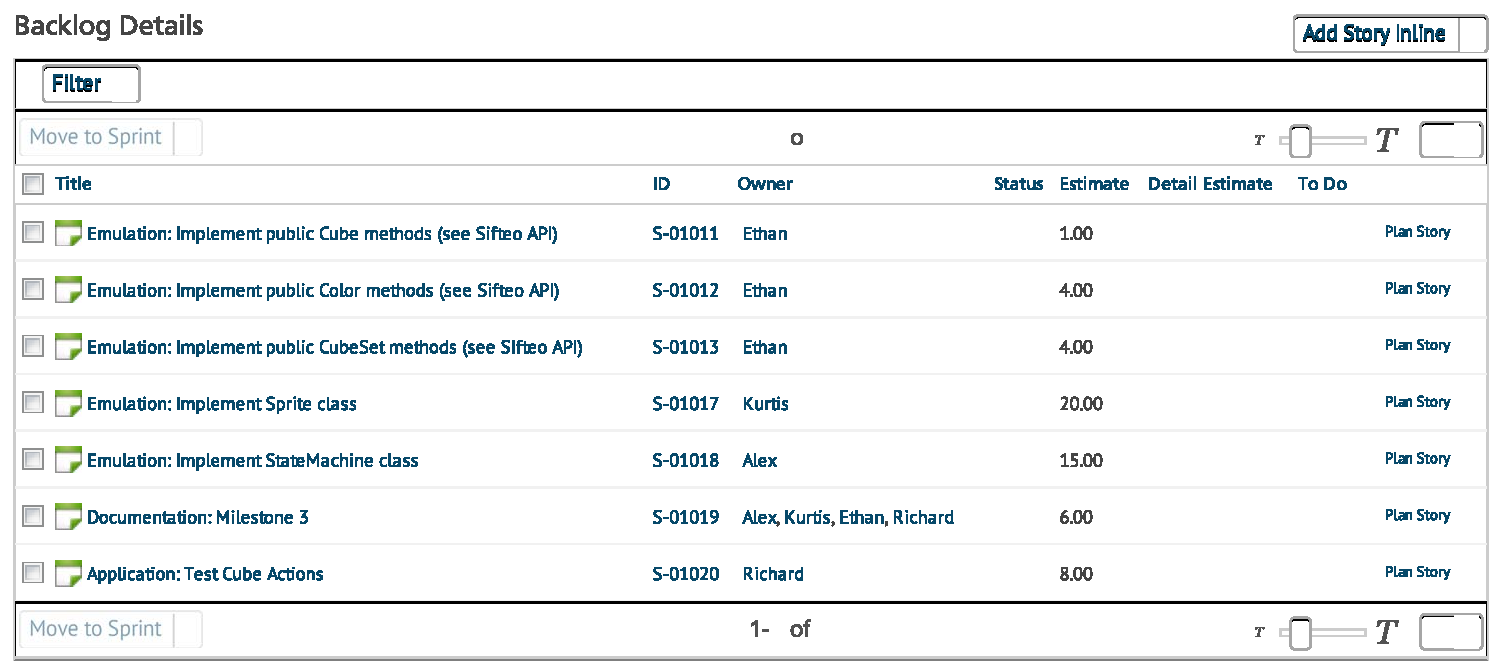
\includegraphics[scale=.63]{pdfs/MS2VersionOne/NewSprintBacklog_cropped.pdf}

This sprint's work will include finishing out a few classes in the Sifteo namespace and implementing two classes from the Sifteo.Util namespace (Sprite and StateMachine). Additionally, we will be writing an application that will be used to test the cube manipulation event handlers written in the last sprint, and those handlers will be tweaked as necessary.

\section*{Class Diagram Before}
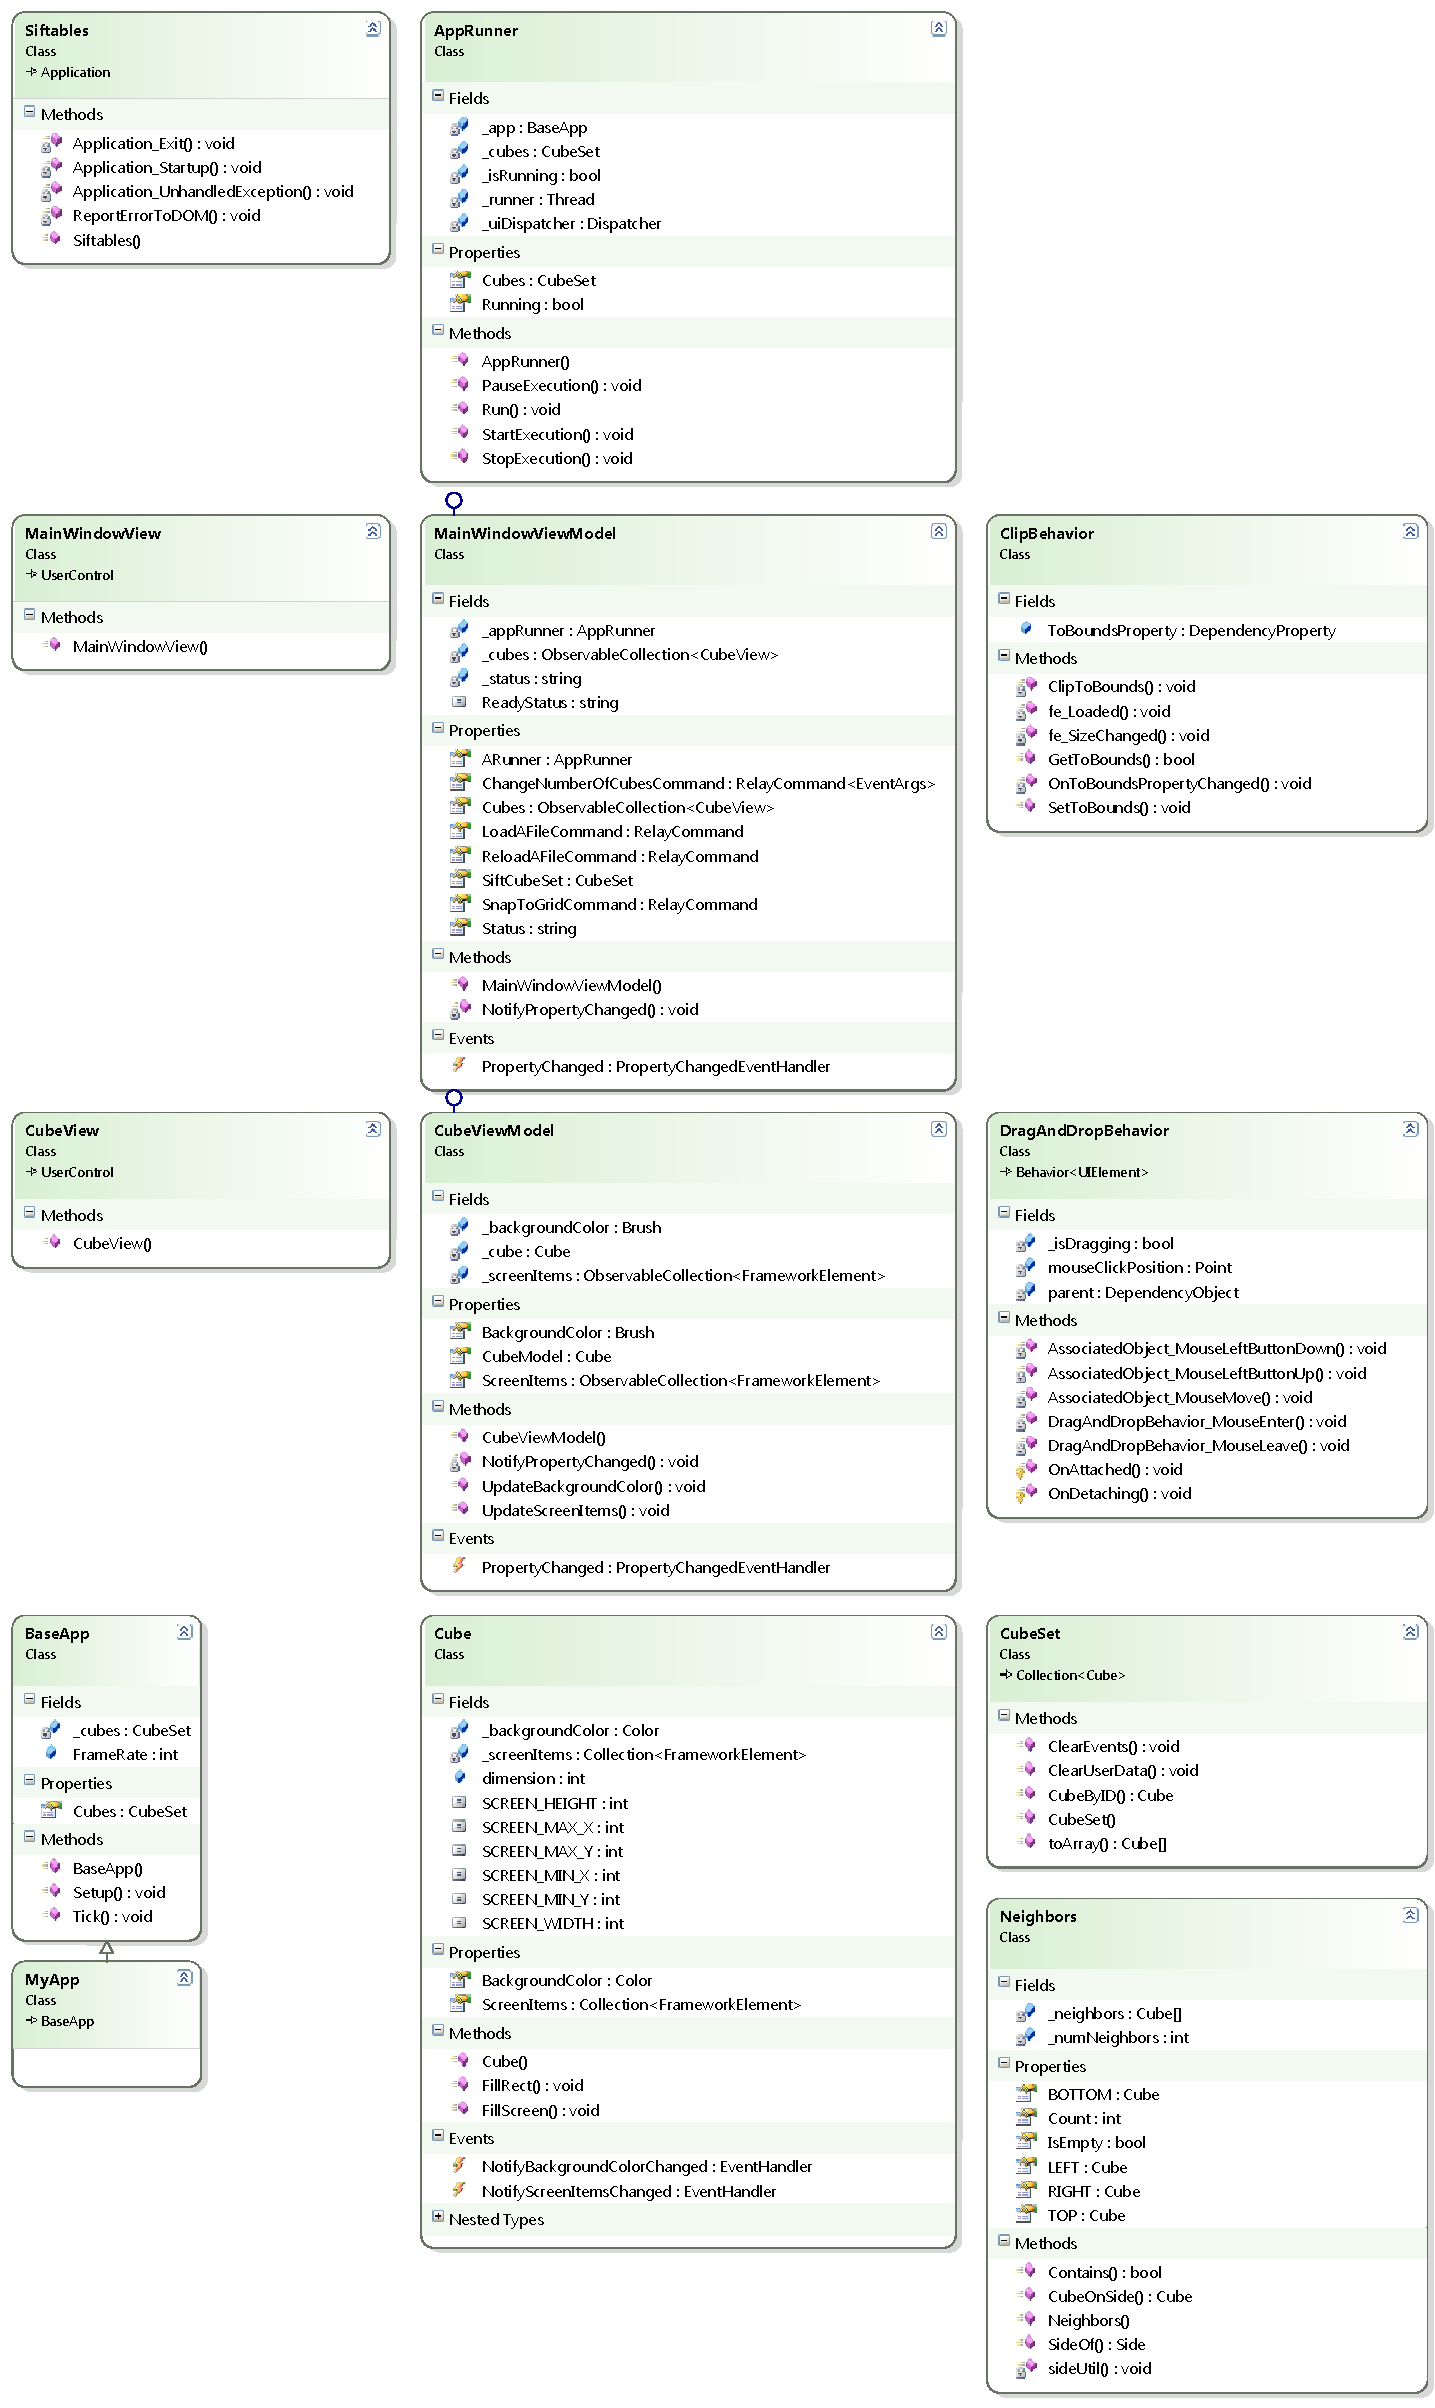
\includegraphics[scale=.6]{pdfs/374docs/MS5Models/ClassDiagram_cropped.pdf}
%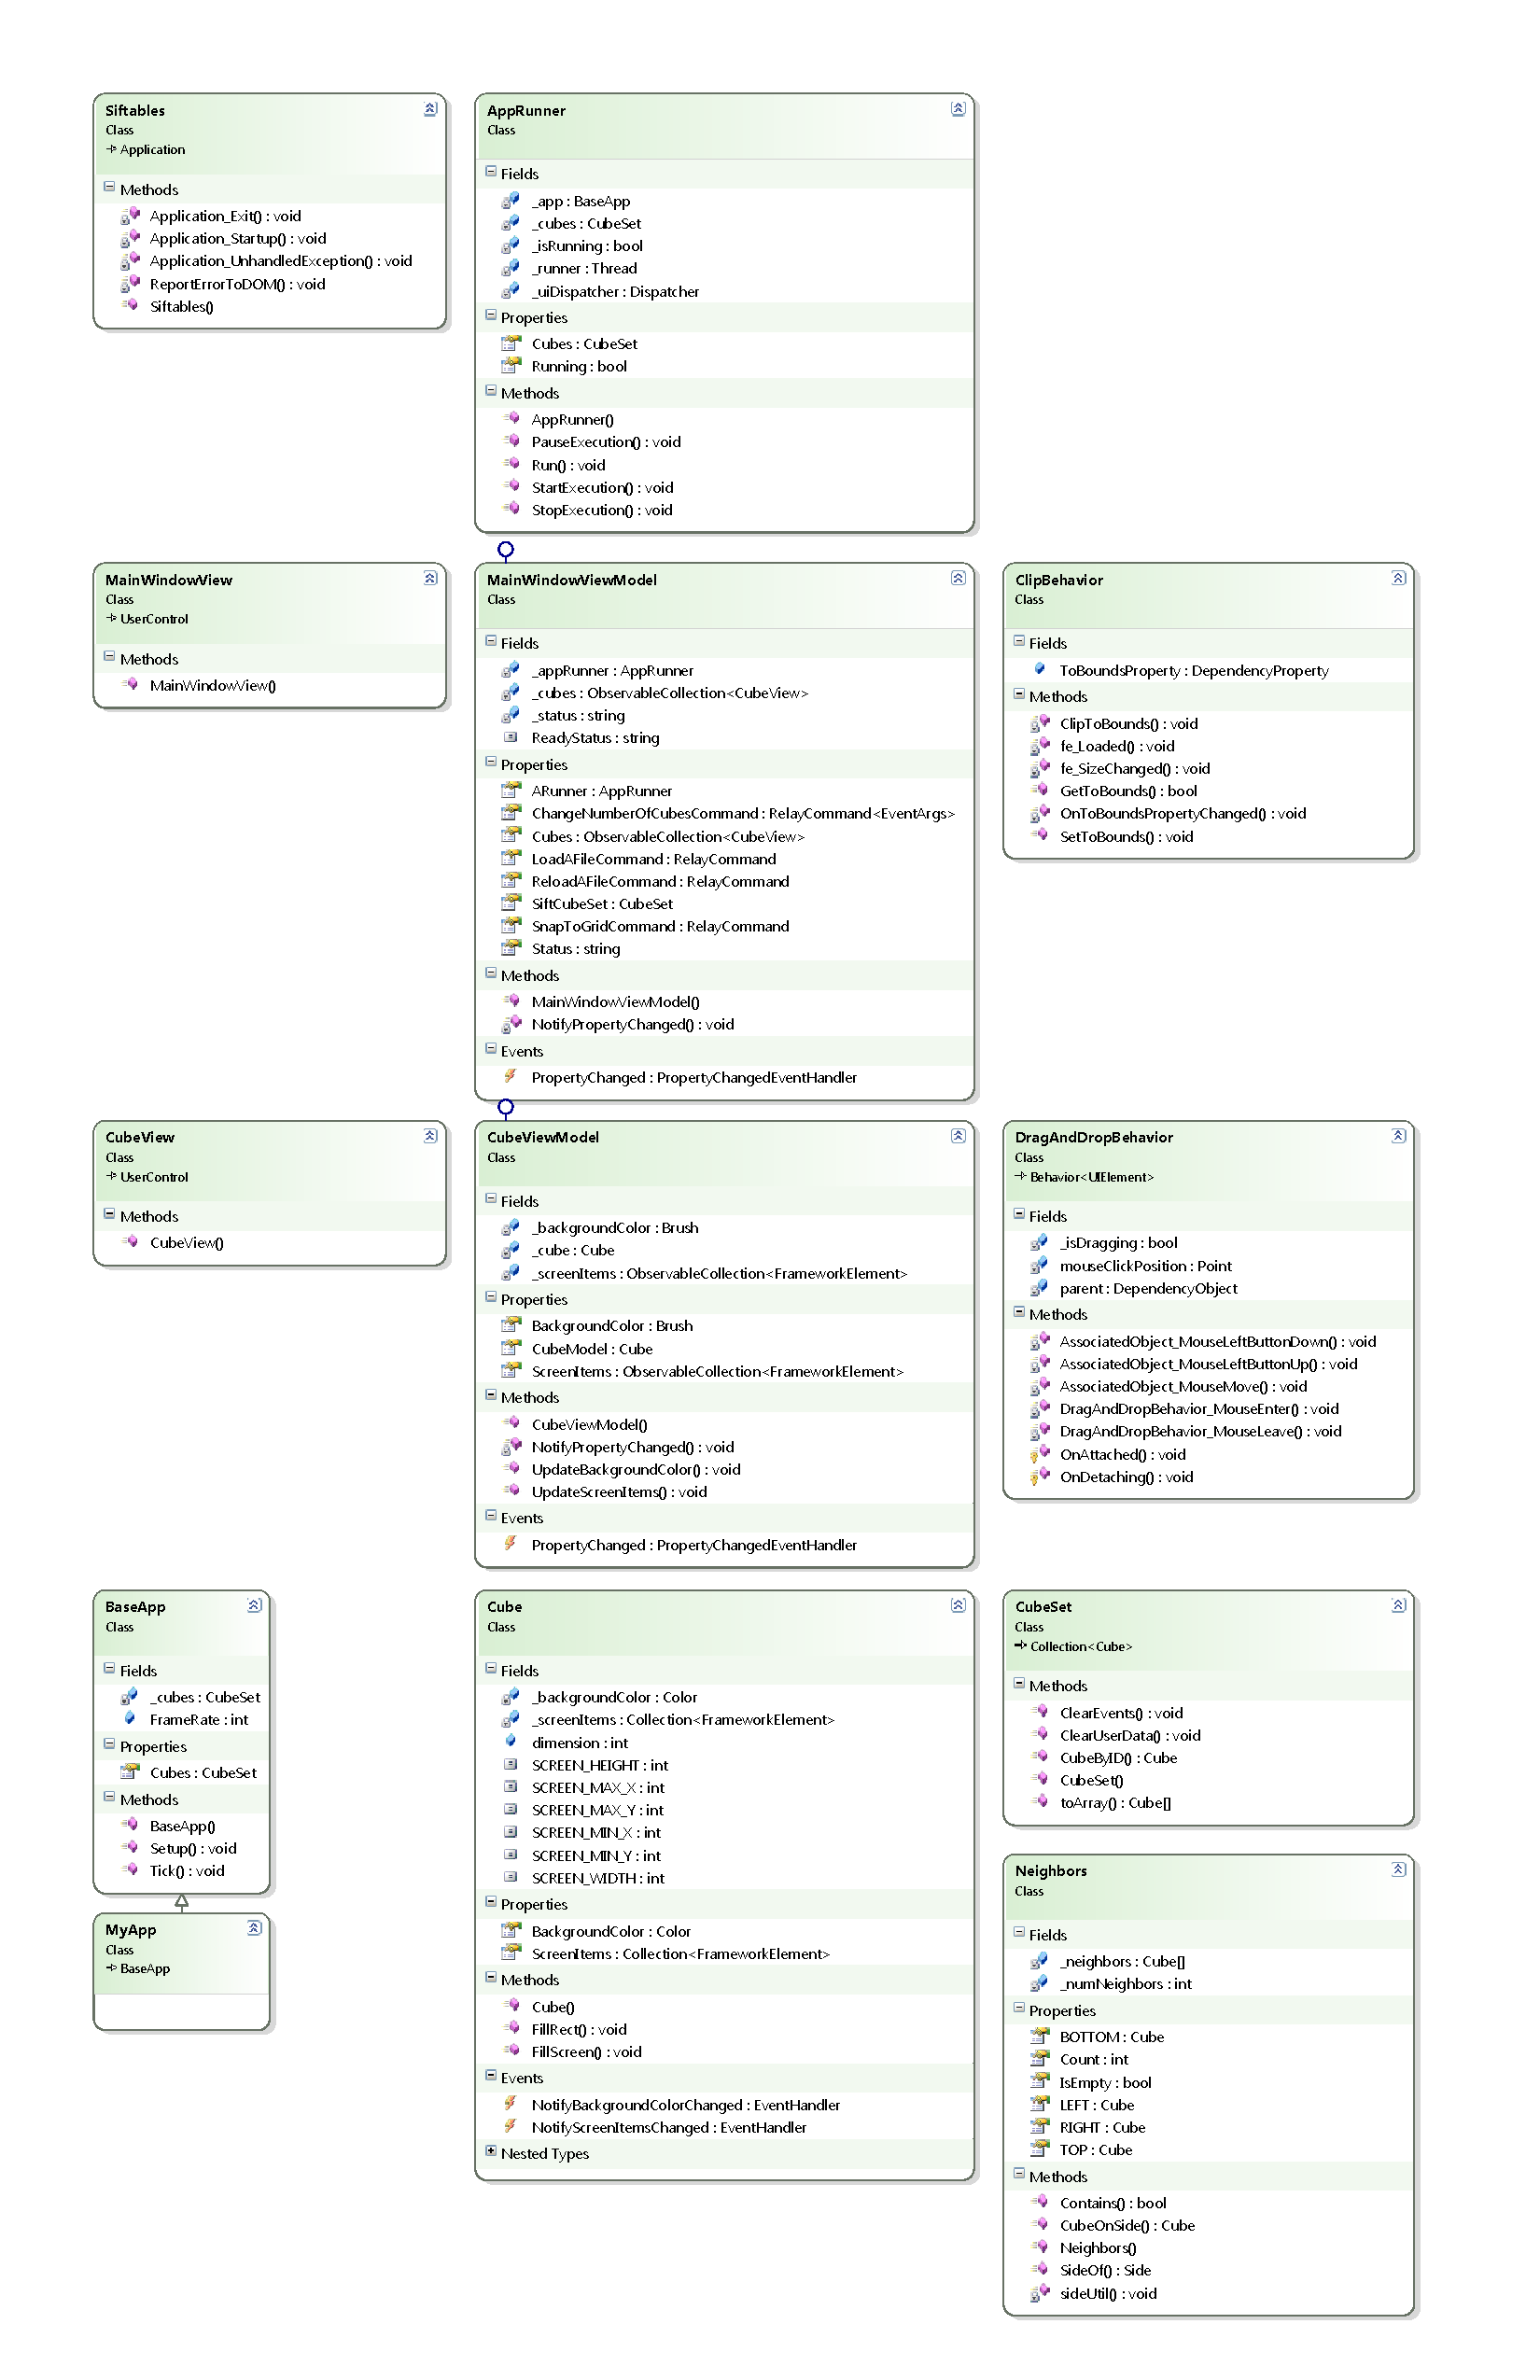
\includegraphics[scale=.6]{pdfs/374docs/MS5Models/ClassDiagram.pdf}

\subsection*{After}
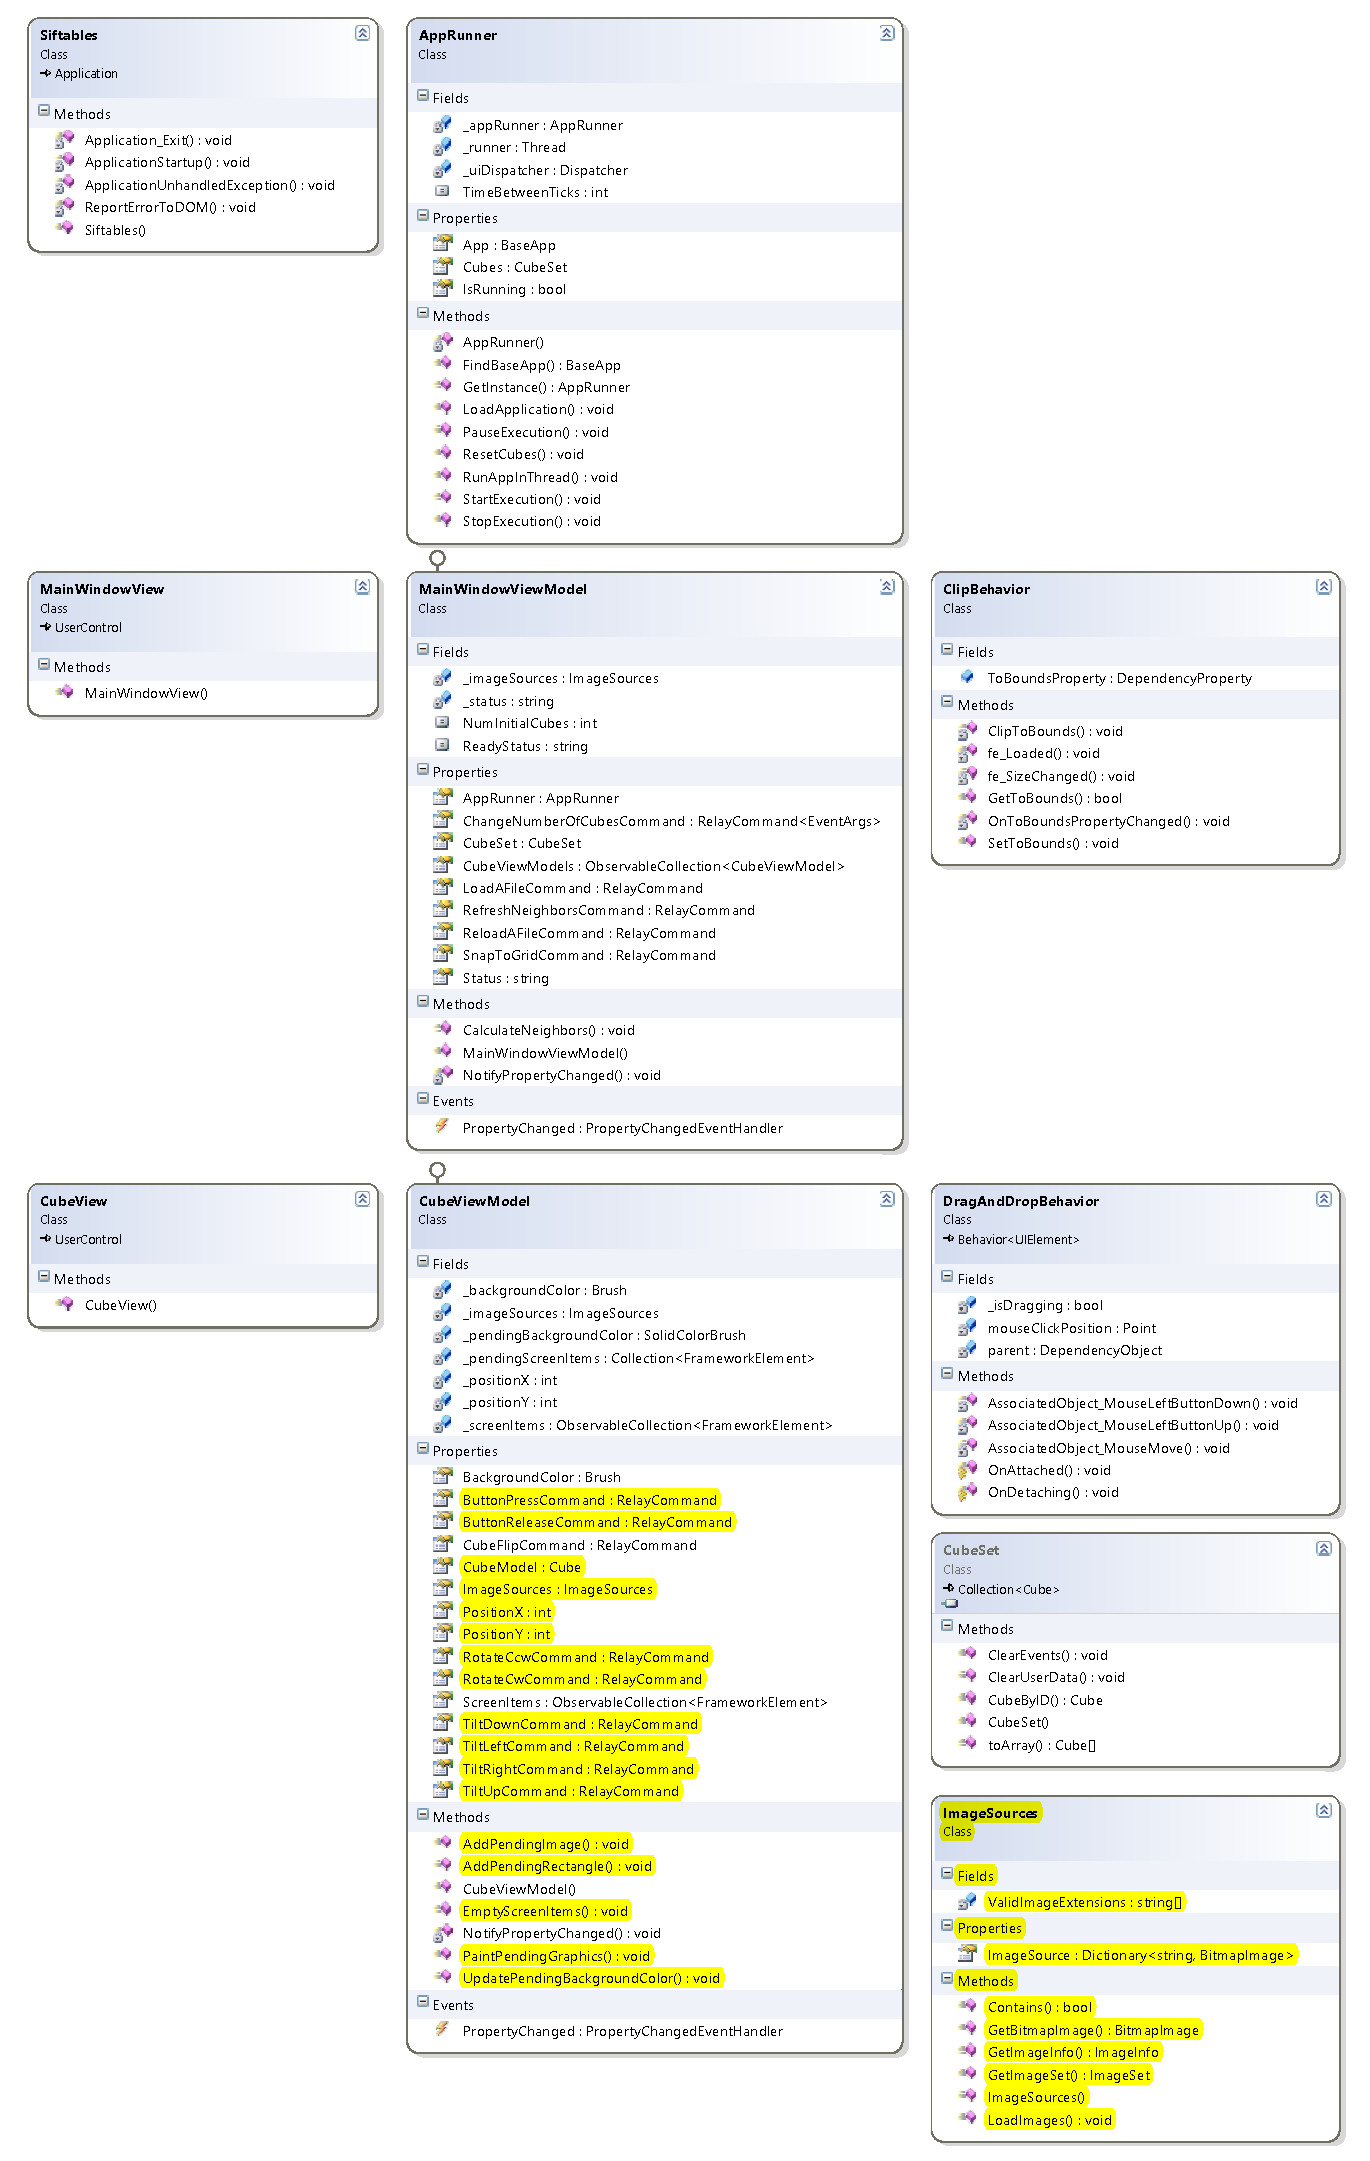
\includegraphics[scale=.85]{pdfs/SiftablesClassDiagram.png}
\clearpage
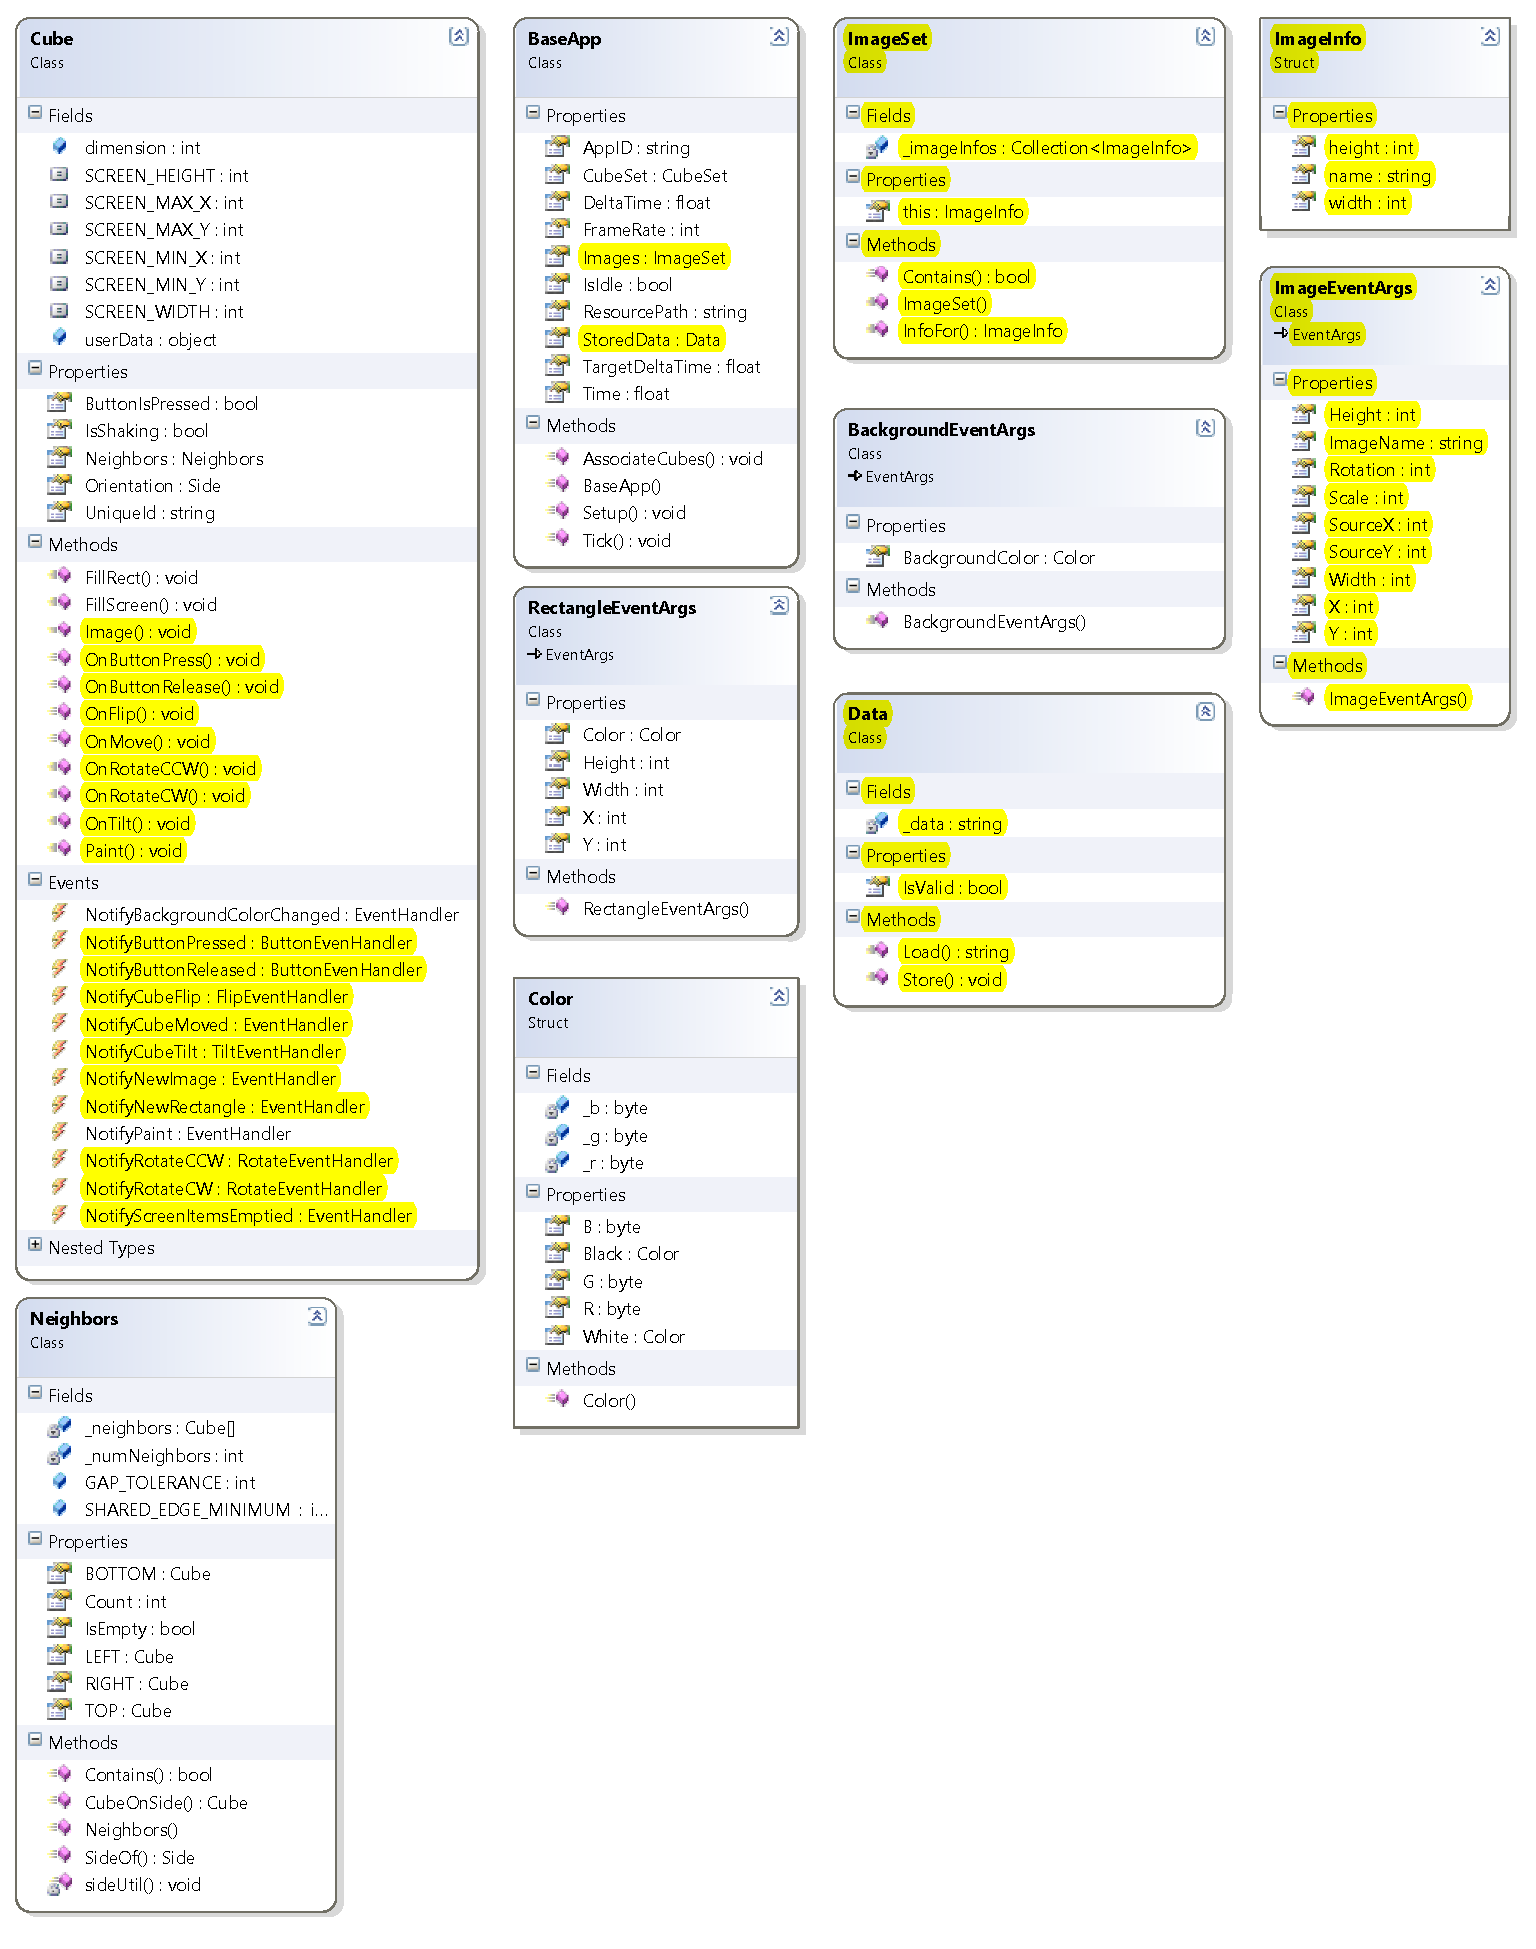
\includegraphics[scale=.8]{pdfs/SifteoClassDiagram.png}

\clearpage

\section*{Struggle with Code Inertia}
Implementing the Cube.Image() method presented a challenge due to the original structure of our viewmodels. \\

For an image to be rendered to a cube's screen, and in order to mimic the structure we had in place for background color and rectangles, we needed to carry out the following sequence of events: \\
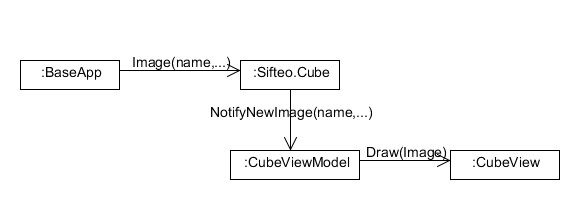
\includegraphics[scale=.8]{pdfs/MS2CodeInertiaDiagram.png}

CubeViewModel is an observer of its Cube (Sifteo model domain), which notifies all subscribers when FillScreen, FillRect, and Image are called from an application. The CubeView (Silverlight UI) is then bound to the collection of graphical elements which the CubeViewModel maintains, so what may be interpreted as method calls above are really notifications (except for the case of Image(name...). \\

This worked well for background colors or rectangles, but images introduce the notion of assets which are associated with an application. \\

When an application is loaded, each of the images in that application's assets directory is loaded in to an ImageSources collection, and any image to be rendered on a cube must come from that collection. We have a class ImageSources which is responsible for loading and making available the image assets, so each CubeViewModel must have a reference to these image sources. Because applications are loaded in MainWindowViewModel (through the AppRunner), the image assets are also loaded at that time (when the application directory is still available). At this point, each of the CubeViewModels needs to have the ability to access those image sources to notify the CubeViews which image to render. \\

This is where our previous structure held us back until some refactoring was done. \\

First of all, the MainWindowView was bound to the MainWindowViewModel, as it should be, and each of the CubeViews was bound to a CubeViewModel, but within the MainWindowViewModel instead of initializing a collection of CubeViewModels, we had initialized a collection of CubeViews. Not only does this volate the principles of MVVM, it does not serve our imaging code either. To access any CubeViewModel, we had to go fetch it from the view, using a call along the lines of \\

(CubeViewModel) cubeView.LayoutRoot.DataContext \\

which reeks of ``Middle Man," ``Message Chain," and ``Inappropriate Intimacy," depending on the vantage point. Instead, we decoupled the CubeViews from the MainWindowViewModel (using some form of ``Remove Middle Man" and separating the layers of our architecture)  so that we never explicitly create a CubeView and instead initialize CubeViewModels and bind the ItemsControl to those viewmodels and use a DataTemplate to indicate to the MainWindowView how we want each viewmodel represented visually. \\

At this point, we had to refactor those DataContext calls to reference the CubeViewModels we now have direct access to, and after this restructuring giving each CubeViewModel access to the set of image sources is much more natural to implement because it can simply be passed from the MainWindowViewModel, where it is created, to the CubeViewModels directly. \\

Although this refactoring added time to this particular task, it will clear the path for the features we are adding in future sprints, because it is expected that we will be implementing sprites and sounds in a similar manner. Now the MVVM structure is correctly preserved, and the classes we have are much more cohesive.

        
\end{document}
